%%%%%%%%%%%%%%%%%%%%%%%%%%%%%%%%%%%%%%%%%
% University Assignment Title Page 
% LaTeX Template
%
% This template has been downloaded from:
% http://www.latextemplates.com
%
% Original author:
% WikiBooks (http://en.wikibooks.org/wiki/LaTeX/Title_Creation)
% 
% Instructions for using this template:
% This title page is presently capable of being compiled as is. This is not 
% useful for including it in another document. To do this, you have two options: 
%
% 1) Copy/paste everything between \begin{document} and \end{document} 
% starting at \begin{titlepage} and paste this into another LaTeX file where you 
% want your title page.
% OR
% 2) Remove everything outside the \begin{titlepage} and \end{titlepage} and 
% move this file to the same directory as the LaTeX file you wish to add it to. 
% Then add \input{./title_page_1.tex} to your LaTeX file where you want your
% title page.
%
%%%%%%%%%%%%%%%%%%%%%%%%%%%%%%%%%%%%%%%%%

%----------------------------------------------------------------------------------------
% PACKAGES AND OTHER DOCUMENT CONFIGURATIONS kljhsdkl
%----------------------------------------------------------------------------------------

\documentclass[letterpaper,12pt]{article}
\usepackage[letterpaper, top = 1 cm, left= 2.2cm, right = 2.2cm ]{geometry}  % Importante para que respete el tamaño de papel
\special{papersize=8.5in,11in}
\usepackage[utf8]{inputenc}
\usepackage{graphicx,setspace}
\usepackage[spanish]{babel}
\usepackage{isomath}
\usepackage{amsmath}
\usepackage{amssymb}
\usepackage{float}
\usepackage{tikz}
\usepackage{todonotes}
\usepackage{subcaption}
\usepackage{listings}
\usepackage{breqn}
\usepackage[nottoc,numbib]{tocbibind}
\usepackage{bm}
\usepackage[T1]{fontenc} 

\usepackage{xcolor,listings}
\usepackage{textcomp}
\lstset{upquote=true}

\setcounter{MaxMatrixCols}{20}
\usepackage{amsfonts}
\newcommand{\Z}{\mathbb{Z}}
\newcommand{\N}{\mathbb{N}}
\newcommand{\F}{\mathbb{F}}

\usepackage{amsthm}
\newcommand{\qedwhite}{\hfill \ensuremath{\Box}}

\newenvironment{spmatrix}[1]
 {\def\mysubscript{#1}\mathop\bgroup\begin{pmatrix}}
 {\end{pmatrix}\egroup_{\textstyle\mathstrut\mysubscript}}

\begin{document}

\author{}
\date{}
\title{Proyecto Final: Base de datos de médicos}

\begin{titlepage}
    \centering
    \vfill
\includegraphics[width=0.8\textwidth]{logoITESM.png} 
 
 \vspace{1 cm}
   {\bfseries \Huge
    \underline{Proyecto Final: Base de datos de médicos}
   }    
    
    \vspace{3 cm} 
    
    {\large
   
        \textbf{Alumnos:}\\
    \vspace{0.3 cm} 
    Salvador Orozco Villalever - A07104218\\
        
        \vspace{0.3 cm} 
    Luis Francisco Flores Romero - A01328937\\
        
        \vspace{0.3 cm} 
    Guillermo Garduño García - A01322809\\
        
        \vspace{0.3 cm}
        Aranzza Abascal Fararoni - A01329203\\
        
        \vspace{1 cm} 

        \textbf{Profesor}:\\
        \vspace{0.3 cm} 
        Dr. David Ricardo Sol Martínez\\ 
        \vspace{1 cm} 

        \textbf{Materia}:\\
        \vspace{0.3 cm} 
        Bases de datos\\
        \vspace{1 cm} 

        \textbf{Fecha de entrega}:\\
        \vspace{0.3 cm} 
        4 de mayo de 2017\\
        \vspace{1 cm}

\textbf{ITESM Campus Puebla}\\
    }
    \vfill
    \vfill
    \vfill
\end{titlepage}

\pagebreak

\tableofcontents

\pagebreak

\section{Descripción del problema}

El proyecto surgió ante a la necesidad del familiar de uno de los integrantes del equipo, quien buscaba un especialista de la salud con carrera reconocida y experiencia comprobable, debido a la naturaleza de la consulta que esta persona deseaba realizar. Lo que sucedió fue que el pariente de nuestro compañero se percató de que la búsqueda de especialistas de la salud no era tarea fácil, pues no existe una base de datos en la que se pueda verificar la calidad de la antención brindada por los médicos. Esto dio lugar al planteamiento de la aplicación: una página web en la que cualquier persona puedaa buscar médicos, escribir reseñas acerca de ellos, leer reseñas y puntuaciones de otros médicos, etc... de manera que, al tener más y mejor información acerca de los especialistas, sea posible tomar una decisión más acertada a la hora de requerir una consulta de uno de ellos.

\section{Alcance del proyecto}

Inicialmente, la idea era desarrollar algo similar a una red social, con un buscador, perfiles de pacientes y doctores, puntuaciones, reseñas, hospitales, entre otras funcionalidades. Sin embargo, el tiempo y la experiencia con desarrollo web fueron limitantes para llevar esta idea la práctica, de manera que la implementación se delimitó quedando de la siguiente manera:

\vspace{0.3 cm}

\textbf{\underline{Secciones implementadas:}}

\begin{enumerate}
\item Registro de médicos y pacientes
\item Buscador de médicos y hospitales
\item Páginas de perfiles de médicos
\item Escritura de reseñas de médicos por parte de los pacientes
\item Aprobación o rechazo de reseñas por parte de los médicos
\end{enumerate}

\vspace{0.3 cm}

\textbf{\underline{Secciones no implementadas:}}

\begin{enumerate}
\item Páginas de perfiles de pacientes
\item Registro de consultorios de médicos
\item Respuesta de los médicos a las reseñas de los pacientes
\item Cierre de sesión
\item Edición de la información del usuario
\end{enumerate}

\section{Casos de uso}

A continuación se presentan los casos de uso realizados previo al desarrollo de la aplicación.

\subsection{Caso 1: Crear usuario}

\begin{figure}[H]
\centering
\includegraphics[width=1\textwidth]{UC-01_Crear_usuario.png}
\caption{\textit{Crear usuario}}
\end{figure}

\subsection{Caso 2: Agregar reseña}

\begin{figure}[H]
\centering
\includegraphics[width=0.80\textwidth]{UC-02_Agregar_resen_a.png}
\caption{\textit{Agregar reseña}}
\end{figure}

\subsection{Caso 3: Editar información de usuario}

\begin{figure}[H]
\centering
\includegraphics[width=0.80\textwidth]{UC-03_Editar_informacio_n_de_usuario.png}
\caption{\textit{Editar información de usuario}}
\end{figure}

\subsection{Caso 4: Buscar médico}

\begin{figure}[H]
\centering
\includegraphics[width=1\textwidth]{UC-04_BuscarMedico.png}
\caption{\textit{Buscar médico}}
\end{figure}

\subsection{Caso 5: Autenticar}

\begin{figure}[H]
\centering
\includegraphics[width=1\textwidth]{UC-05_Autenticar.png}
\caption{\textit{Autenticar}}
\end{figure}

\subsection{Caso 6: Revisar reseñas}

\begin{figure}[H]
\centering
\includegraphics[width=1\textwidth]{UC-06_RevisarResenas.png}
\caption{\textit{Revisar reseñas}}
\end{figure}

\subsection{Caso 7: Responder reseñas}

\begin{figure}[H]
\centering
\includegraphics[width=0.8\textwidth]{UC-07_Responder_resen_a.png}
\caption{\textit{Responder reseñas}}
\end{figure}

\subsection{Caso 8: Aprobar reseñas}

\begin{figure}[H]
\centering
\includegraphics[width=1\textwidth]{UC-08_Aprobar_resen_a.png}
\caption{\textit{Aprobar reseñas}}
\end{figure}

\section{Diagramas}

\subsection{Diagrama Entidad/Relación}
\begin{figure}[H]
\centering
\includegraphics[width=1\textwidth]{UC-08_Aprobar_resen_a.png}
\caption{\textit{Aprobar reseñas}}
\end{figure}

\subsection{Diagrama Relacional}

\subsubsection{Glosario asociado al diagrama relacional}

\section{Queries utilizadas}

\subsection{Búsqueda de un médico}

\subsubsection{A través de su nombre}

\textbf{\underline{En lenguaje natural}}

\vspace{0.3 cm}

Se busca dentro de la tabla doctors a todos los doctores que tengan el nombre dado "search_first_name".

\vspace{0.3 cm}

\textbf{\underline{En SQL}}

\vspace{0.3 cm}

\begin{lstlisting}[
           language=SQL,
           showspaces=false,
           basicstyle=\ttfamily,
           numbers=left,
           numberstyle=\tiny,
           commentstyle=\color{gray}
        ]
SELECT * 
FROM doctors
WHERE doctors.first_name = search_first_name;
\end{lstlisting}

\subsubsection{A través de su apellido}

\textbf{\underline{En lenguaje natural}}

\vspace{0.3 cm}

Se busca dentro de la tabla doctors a todos los doctores que tengan el apellido dado "search_last_name".

\vspace{0.3 cm}

\textbf{\underline{En SQL}}

\vspace{0.3 cm}

\begin{lstlisting}[
           language=SQL,
           showspaces=false,
           basicstyle=\ttfamily,
           numbers=left,
           numberstyle=\tiny,
           commentstyle=\color{gray}
        ]
SELECT * 
FROM doctors
WHERE doctors.last_name = search_last_name;
\end{lstlisting}

\subsubsection{A través de su especialidad}

\textbf{\underline{En lenguaje natural}}

\vspace{0.3 cm}

Debido a que la especialidad se encuentra en una tabla distinta, es necesario realizar una query donde busquemos el id de la especialidad dada, para posteriormente buscar dentro de doctors a todos los doctores que cuenten con esa especialidad.

\vspace{0.3 cm}

\textbf{\underline{En SQL}}

\vspace{0.3 cm}

\begin{lstlisting}[
           language=SQL,
           showspaces=false,
           basicstyle=\ttfamily,
           numbers=left,
           numberstyle=\tiny,
           commentstyle=\color{gray}
        ]
SELECT * 
FROM doctors 
WHERE doctors.specialty_id = (
      SELECT specialties.id
            FROM specialties
            WHERE specialties.name = search_specialty);
\end{lstlisting}

\subsubsection{A través de su cédula}

\textbf{\underline{En lenguaje natural}}

\vspace{0.3 cm}

Se busca dentro de la tabla doctors al doctor que tengan la cédula dada "search_medical_id".

\vspace{0.3 cm}

\textbf{\underline{En SQL}}

\vspace{0.3 cm}

\begin{lstlisting}[
           language=SQL,
           showspaces=false,
           basicstyle=\ttfamily,
           numbers=left,
           numberstyle=\tiny,
           commentstyle=\color{gray}
        ]
SELECT * 
FROM doctors
WHERE doctors.medical_id = search_medical_id;
\end{lstlisting}

\subsection{Búsqueda de un hospital}

\subsubsection{A través de su nombre}

\textbf{\underline{En lenguaje natural}}

\vspace{0.3 cm}

Se busca dentro de la tabla hospitals al hospital que tengan el nombre dado "search_name".

\vspace{0.3 cm}

\textbf{\underline{En SQL}}

\vspace{0.3 cm}

\begin{lstlisting}[
           language=SQL,
           showspaces=false,
           basicstyle=\ttfamily,
           numbers=left,
           numberstyle=\tiny,
           commentstyle=\color{gray}
        ]
SELECT * 
FROM hospitals
WHERE hospitals.name = search_name;
\end{lstlisting}

\subsubsection{A través de su ciudad}

\textbf{\underline{En lenguaje natural}}

\vspace{0.3 cm}

Debido a que la ciudad se encuentra en una tabla distinta, es necesario realizar una query donde busquemos el id de la ciudad dada, para posteriormente buscar dentro de hospitals todos los hospitales que se encuentren en esa ciudad.

\vspace{0.3 cm}

\textbf{\underline{En SQL}}

\vspace{0.3 cm}

\begin{lstlisting}[
           language=SQL,
           showspaces=false,
           basicstyle=\ttfamily,
           numbers=left,
           numberstyle=\tiny,
           commentstyle=\color{gray}
        ]
SELECT * 
FROM hospitals 
WHERE hospitals.id = (
      SELECT cities.id
            FROM cities
            WHERE cities.name = search_name);
\end{lstlisting}

\section{Transacciones utilizadas}

\subsection{Al tratar de ingresar una reseña}

\section{Reflexión sobre el impacto del proyecto en el contexto social}

\subsection{Reflexión de Salvador Orozco Villalever - A07104218}

Yo considero que este proyecto fue muy interesante pues nos permitió poner en práctica por primera vez un sistema de información a través de una base de datos y una aplicación a la cual miles y miles de personas podrían tener acceso potencialmente. Creo que el tema que elegimos (los servicios de salud) es excelente y de gran importancia, pues es precisamente en este ámbito en el cual hace falta mucho en nuestro país. Por otro lado, considero que ideas como aquella en la que se basó este proyecto son muy valiosas en la industria de los servicios, pues creo que para tomar decisiones correctas en situaciones como \textit{"¿A qué especialista acudir en caso de presentar una urgencia médica?"}, hay que tener la información adecuada, además de que ésta debe provenir de fuentes confiables y de primera mano. En nuestro caso, decidimos que los mismos pacientes serían la mejor fuente de información, por lo que son sus comentarios y calificaciones los que se almacenan en nuestra base de datos. 

\vspace{0.3 cm}

Si bien no logramos desarrollar todo lo que en un principio imaginamos que nuestra aplicación podría realizar, me siento satisfecho por haber logrado terminar una primera parte que brinda al usuario una experiencia básica de lo que éste podría ser capaz de hacer en la aplicación completa. Creo que en un futuro esta aplicación podría ser desarrollada por completo y que ésta podría llegar a ser muy popular. Sin embargo, considero que para lograr lo anterior tendríamos que seguir excelentes prácticas de ingeniería de software, además de aprender más acerca de 
desarrollo web. 

\vspace{0.3 cm}

Definitivamente, el área de sistemas de información se ha convertido en mi área favorita dentro de las TIs, no sólo porque hay tanto por hacer y por mejorar en este ámbito, sino porque además, se trata de un área en la cual el desarrollo de aplicaciones y tecnologías puede tener un gran impacto social.

\subsection{Reflexión de Guillermo Garduño García - A01322809}
Personalmente considero que realizar este proyecto fue una buena manera de poner en práctica los temas vistos en clase. El reto de realizar una aplicación funcional que tenga conexión con una base de datos, no ayudo a aprender sobre temas adicionales a lo visto en el curso. Considero que nuestro proyecto es una idea que podría significar una gran ayuda para toda la sociedad. El poder buscar médicos especialistas y poder tomar la decisión de con cual asistir con base a información verdadera. Si bien la idea es bastante buena, creo que existen muchos riesgos, principalmente por la sociedad en la que vivimos, corriendo riesgos de que la información no sea completamente verídica o que busque beneficiar o dañar a cierto médico. Aun así, es una aplicación que busca ayudar a todas las personas y creo que puede hacerlo.

\vspace{0.3 cm}

Finalmente considerando que siendo nuestra primera aplicación web, logramos crear un prototipo funcional, que muestra nuestra idea original y que gracias a su conexión con la base de datos podemos realizar registros de pacientes y médicos para después poder escribir reseñas y consultar información de los doctores. Así es que me siento conforme con lo obtenido de este proyecto y con la idea de que puede mejorar y ser un buen proyecto a futuro.

\section{Anexos}

\subsection{Capturas de pantalla de la página web}

\begin{figure}[H]
\centering
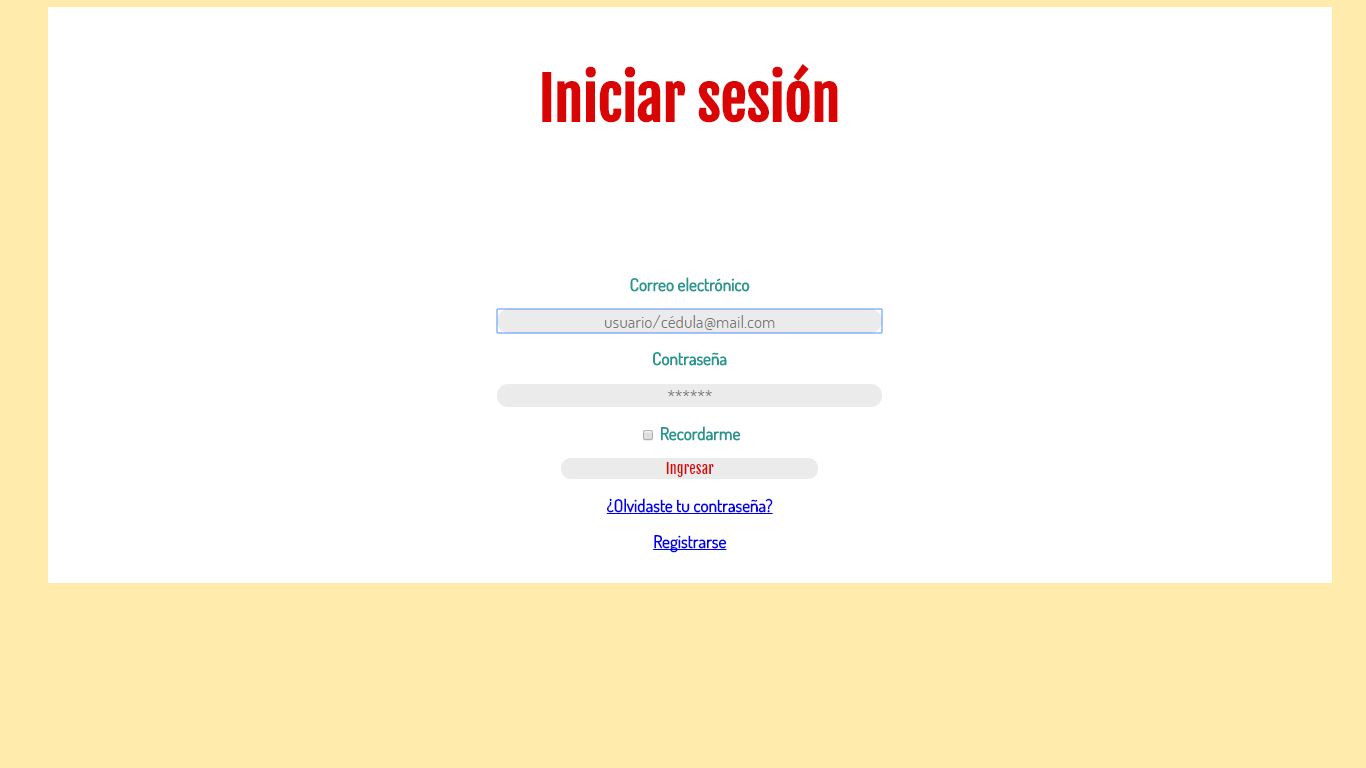
\includegraphics[width=0.8\textwidth]{1_InicioDeSesion.png}
\caption{\textit{Inicio de sesión}}
\end{figure}

\begin{figure}[H]
\centering
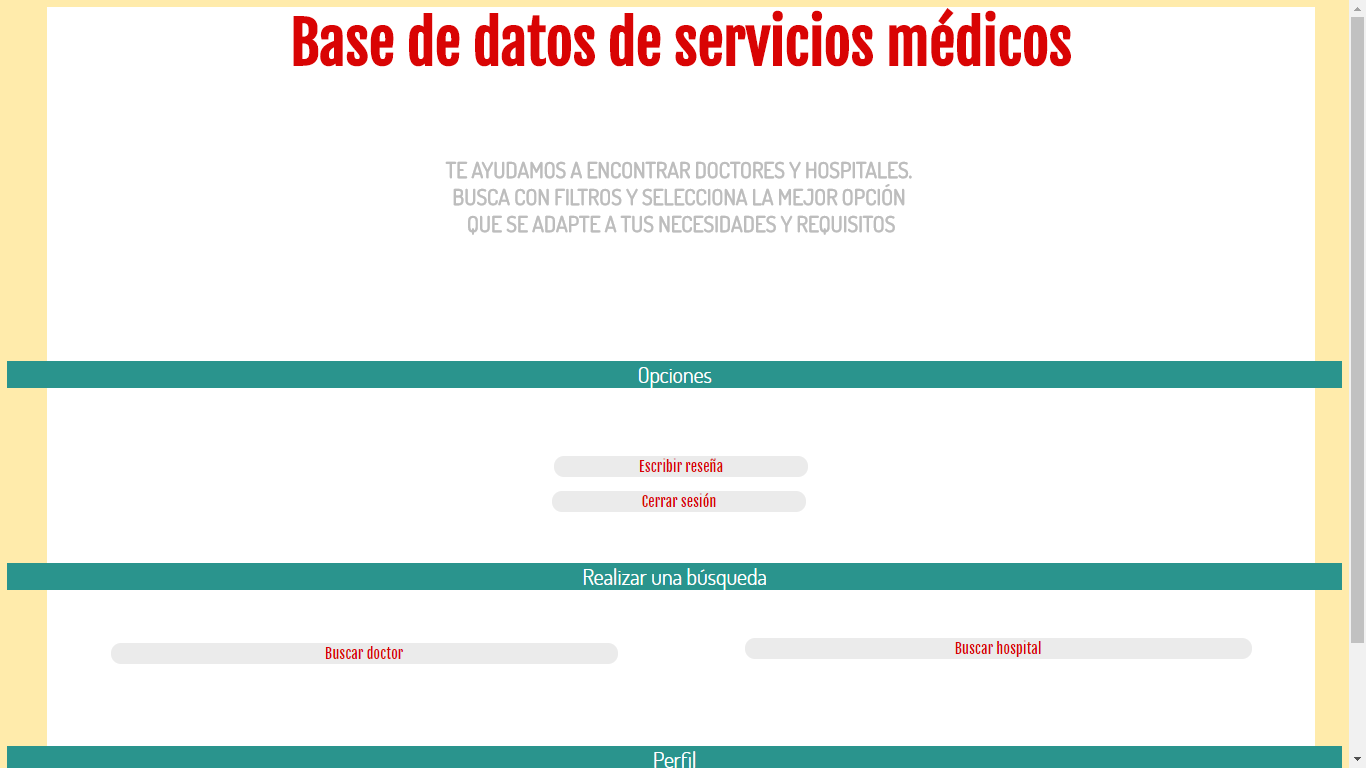
\includegraphics[width=0.8\textwidth]{2_PaginaPrincipal.png}
\caption{\textit{Página principal}}
\end{figure}

\begin{figure}[H]
\centering
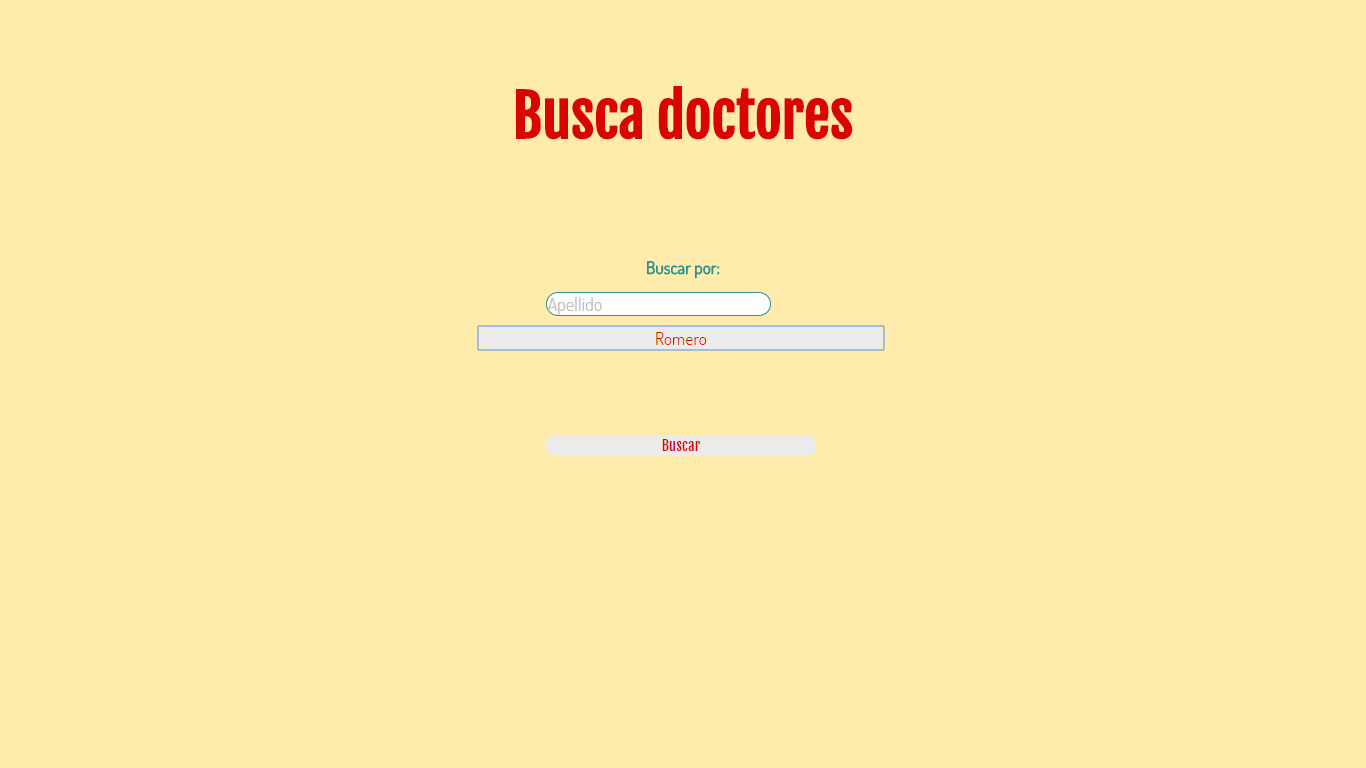
\includegraphics[width=0.8\textwidth]{3_BusquedaDeDoctores.png}
\caption{\textit{Búsqueda de doctores}}
\end{figure}

\begin{figure}[H]
\centering
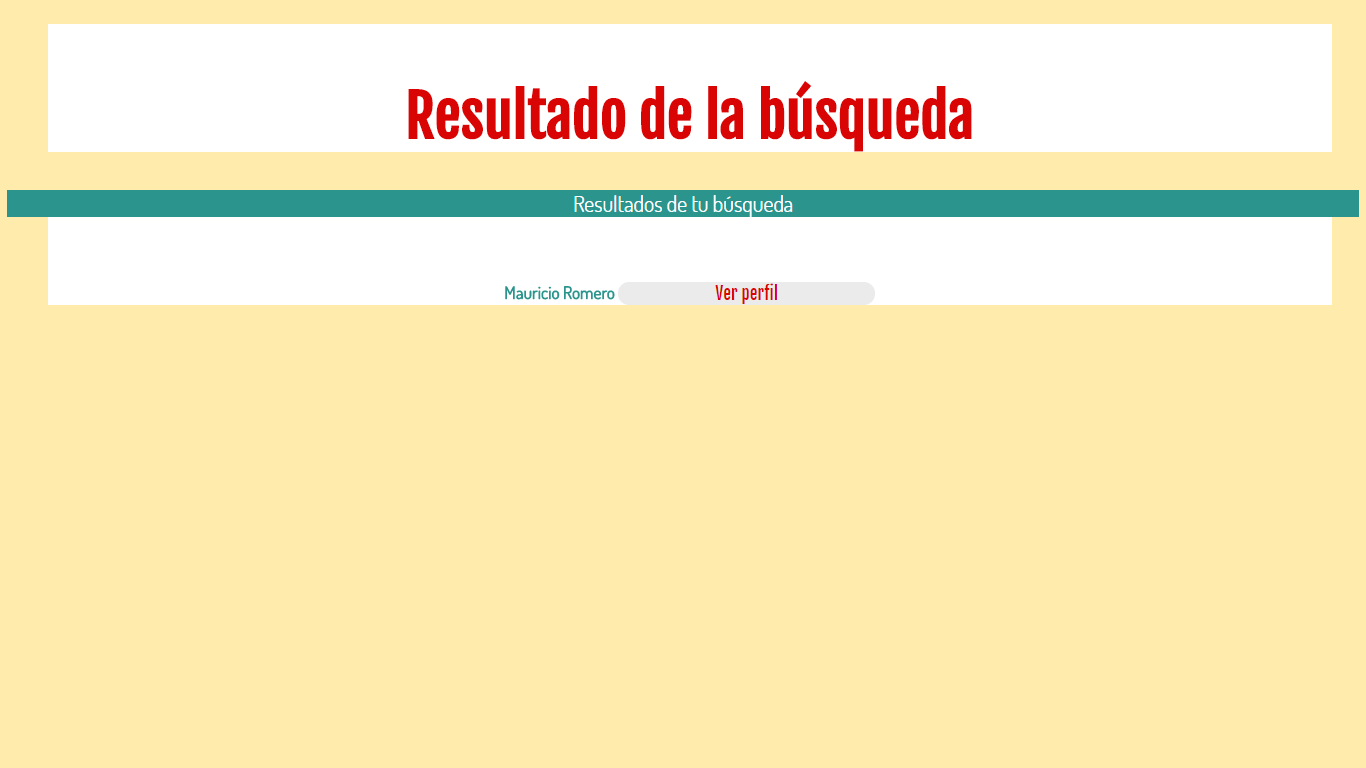
\includegraphics[width=0.8\textwidth]{4_ResultadoDeLaBusquedaDeDoctores.png}
\caption{\textit{Resultados de la búsqueda de doctores}}
\end{figure}

\begin{figure}[H]
\centering
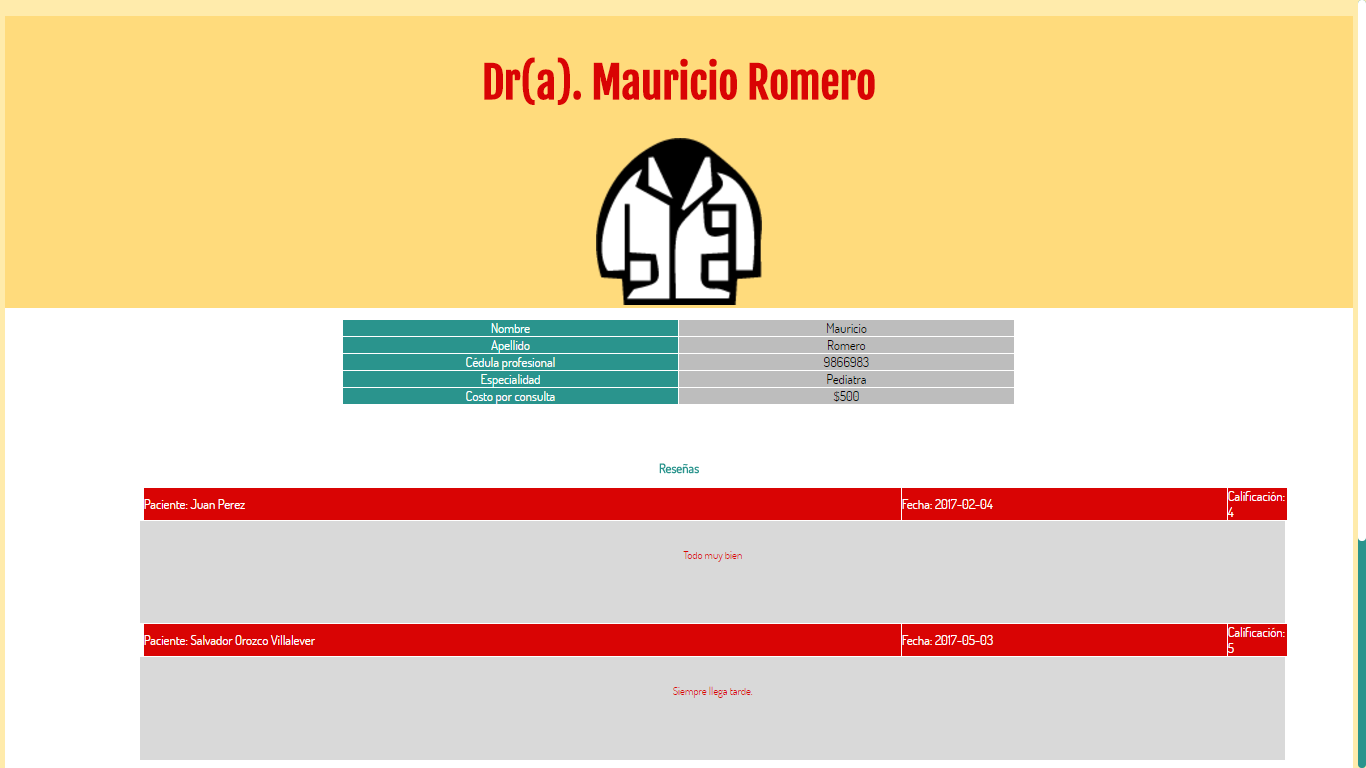
\includegraphics[width=0.8\textwidth]{5_PerfilDeUnDoctor.png}
\caption{\textit{Perfil de un doctor}}
\end{figure}

\begin{figure}[H]
\centering
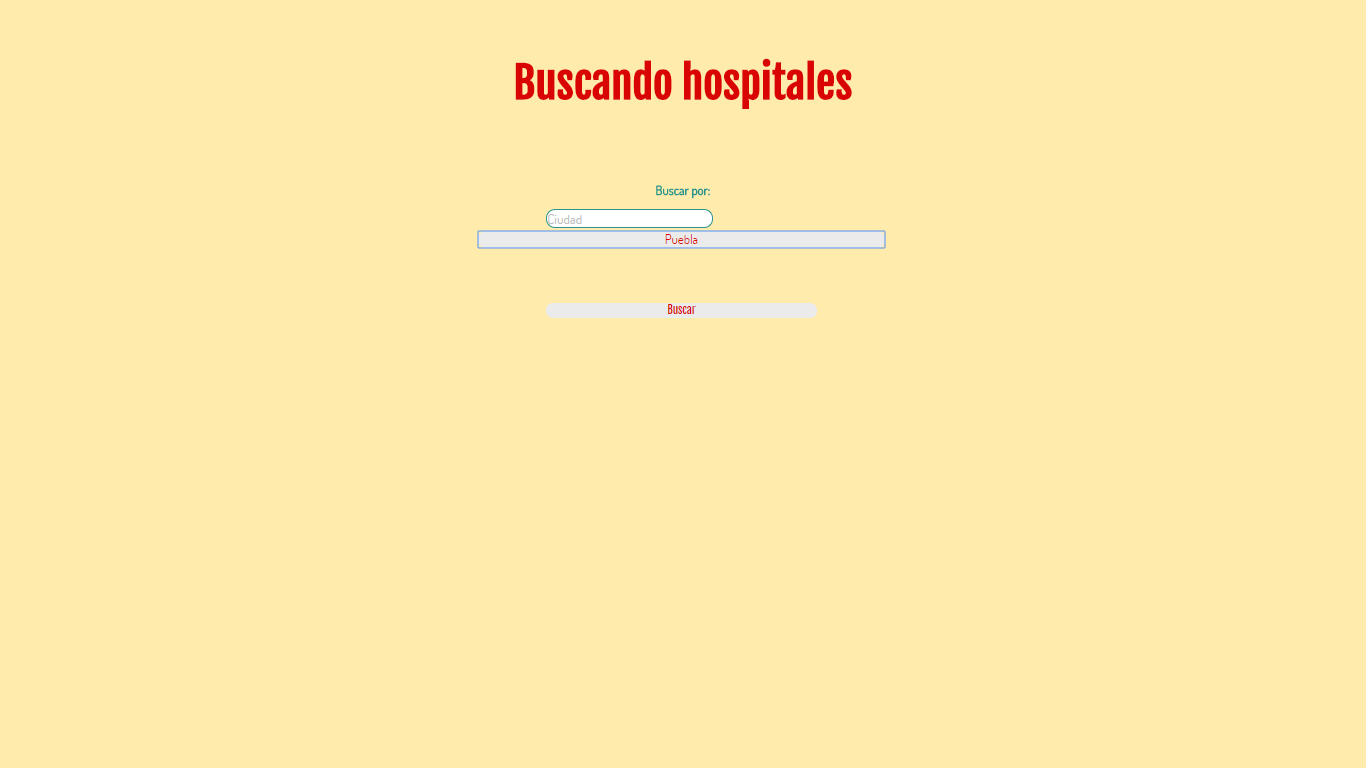
\includegraphics[width=0.8\textwidth]{6_BusquedaDeHospitales.png}
\caption{\textit{Búsqueda de hospitales}}
\end{figure}

\begin{figure}[H]
\centering
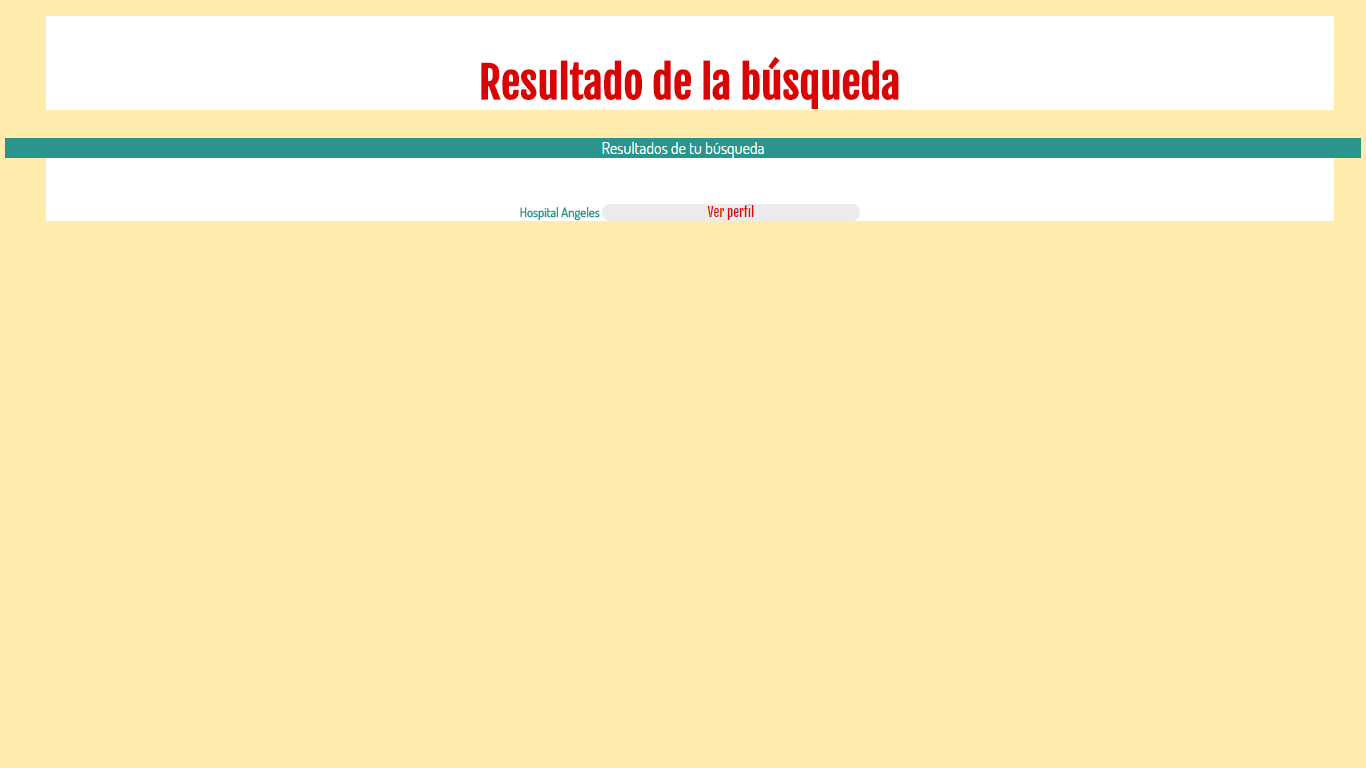
\includegraphics[width=0.8\textwidth]{7_ResultadoDeLaBusquedaDeHospitales.png}
\caption{\textit{Resultado de la búsqueda de hospitales}}
\end{figure}

\begin{figure}[H]
\centering
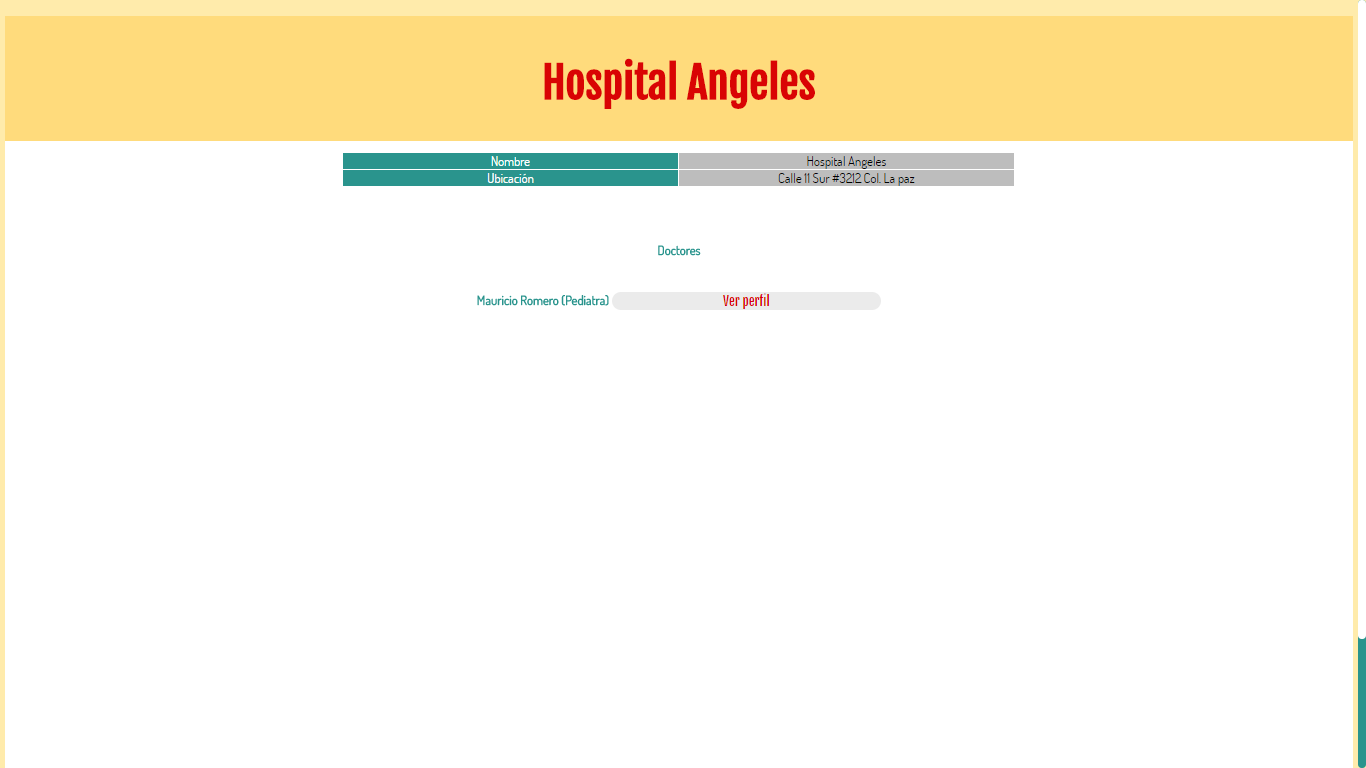
\includegraphics[width=0.8\textwidth]{8_PerfilDelHospital.png}
\caption{\textit{Perfil de un hospital}}
\end{figure}

\begin{thebibliography}{1}

\bibitem{notes1} Elmasri, R., Navathe, S. B. (2007). Fundamentals of Database Systems (5th ed.). Reading, MA: Addison-Wesley.

\bibitem{notes2} It's Kinda Like Netflix for Your Career! (2015) Laracasts (n.d.). Consultado el 4 de mayo de 2017 en  https://laracasts.com/

\end{thebibliography}

\end{document}